\section{Aufbau}
\label{sec:Aufbau}
Auf Bild \ref{} ist der Versuchsaufbau zu sehen. Der Rezipient () ist mit der Turbomolekularpumpe (P2) verbunden, 
welche wiederum mit der Drehschieberpumpe (P1) verbunden ist. Über das Ventil (V1) kann die Drehschieberpumpe vom 
restlichen Aufbau abgeschiebert werden. Das selbe ist Für die Turbopumpe mit dem Ventil (V2) möglich.
Zum Belüften des Rezipienten sind ein Ventil (V3) und ein Drosselventi (D1) mit dem Rezipienten verbunden.
Die für den Versuch genutzten Messgeräte sind zum einen das Pirani-Kaltkathoden-Vakuumeter (M1) zur Bestimmung der 
von der Turbopumpe erzeugten Drücke und das Piezo-Pirani-Vakuumeter (M2) für die Drücke, die durch die Drehschieberpumpe 
erzeugt werden.

    \begin{figure}
        \centering
        \caption{SVersuchsaufbau.}
        \label{fig:Versuchsaufbau}
        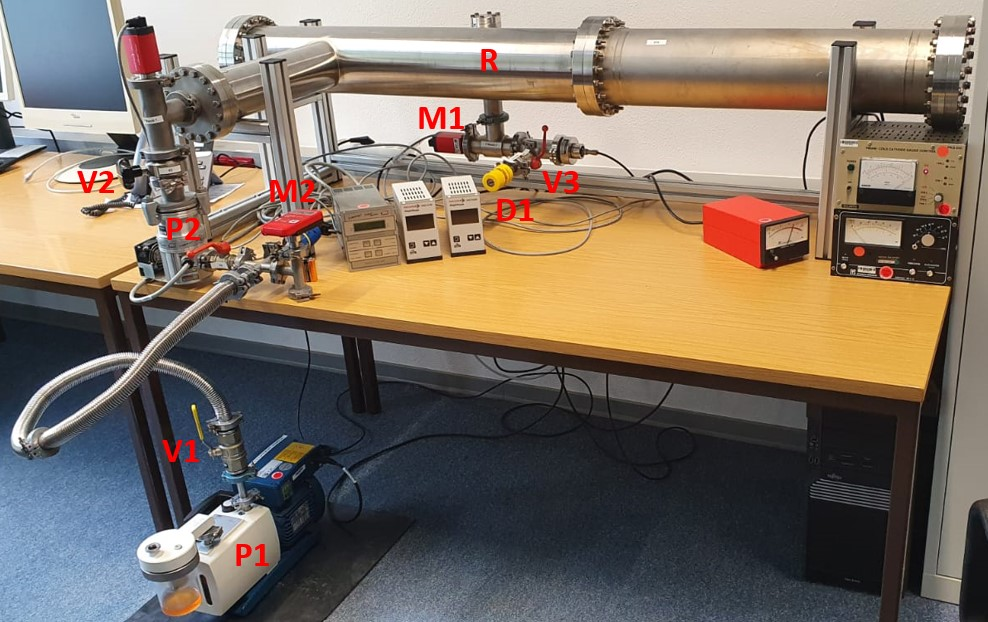
\includegraphics[width=0.6\textwidth]{Versuchsaufbau_V70.jpeg}
    \end{figure}


\section{Durchführung}
\label{sec:Durchführung}
Bevor die eigentlichen Messungen beginnen können, muss überprüft werden ob die Anlage dicht ist.
Dafür wird der Rezipient evakuiert und festgestellt ob der Enddruck im Bereich der entsprechenden Pumpe liegt. 
Ist dies nicht der Fall, muss die Apperatur überprüft werden und undichte stellen abgedichtet werden.

\subsection{Turbomolekularpumpen Messungen}
\label{sec:Turbomolekularpumpen Messungen}
Da die Turbomolekularpumpe schon vor Beginn des Versuchs lief, wurde mit der Bestimmung der Saugleistung der Turbopumpe begonnen.

\subsubsection{Evakuierungskurve}
\label{sec:Evakuierungskurve1}
Zur bestimmung der Evakuierungskurve laufen beide Pumpen und die Ventile zum Rezipienten sind geöffnet.
Nun wird der Rezipient vorsichtig mit geöffnetem V3 und über das Drosselventil D1 belüftet, bis der Druck im Rezipienten bei $p_0 = 5 \dot 10^{-3}$ liegt.
Anschließend wird V3 geschlossen und für 120s alle 10s der Druck im Rezipienten abgelesen.
Diese Prozedur wird drei mal durchgeführt.

\subsubsection{Leckratenmessung}
\label{sec:Leckratenmessung1}
Für die Leckratenmessung wird bei laufenden Pumpen und geöffneten V1 und V2 über das Drosselventil ein Gleichgewichtsdruck eingestellt.
Danach wird die Turbomolekularpumpe durch schließen des Ventils V2 abgeschiebert und 120s lang alle 10s der Druck gemessen.
Dies wird insgesammt 3 mal pro Gleichgewichtsdruck und mit vier verschiedenen Gleichgewichtsdrücken ($p_g = 5 \dot 10^{-5}; 7 \dot 10^{-5}; 1 \dot 10^{-4}; 2 \dot 10^{-4} mbar$) durchgeführt.

\subsection{Drehschieberpumpen Messungen}
\label{sec:Drehschieberpumpen Messungen}
Für die Bessungen mit der Drehschieberpumpe wird die Turbomolekularpumpe ausgestellt. Das Ventil V2 bleibt die gsamte Zeit geöffnet.

\subsubsection{Evakuierungskurve}
\label{sec:Evakuierungskurve2}
Bei der Bestimmung der Evakuirungskurve der Drehschieberpumpe bleiben V1 und V2 geöffnet, der Rezipient wird über V3 und D1 geflutet, 
bis Atmosphärendruck innerhalb herrscht. Dann wird V3 geschlossen und 600 s lang alle 10 s der Druk im Rezipienten abgelesen.
Auch diese Messung wir drei mal durchgeführt.

\subsubsection{Leckratenmessung}
\label{sec:Leckratenmessung2}
Die Leckratenmessung der Drehschieberpumpe verläuft fast Äquivalent zur Messung mit der Turbomolekularpumpe.
Über das Drosselventil D1 werden vier verschiedene Gleichgewichtsdrücke ($p_g = 0,5; 10; 50; 100 mbar$) eingestellt.
Anschließend wird die Pumpe über V1 abgeschiebert und 200 s alle 10 s der Druck bestimmt. Für jeden Gleichgewichtsdruck 
wird die Messun wieder 3 mal durchgeführt.


